% !TEX encoding = UTF-8
% !TEX TS-program = pdflatex
% !TEX root = ../tesi.tex

%**************************************************************
\chapter{Valutazione Retrospettiva}
\label{cap:valutazione-retrospettiva}
%**************************************************************

\section{Difficoltà incontrate}
\label{sec:difficolta_incontrate}
Le prime difficoltà incontrate a livello personale sono state di tipo tecnologico: non mi ero mai trovato a programmare con linguaggi orientati al \textit{frontend}, e ho dovuto quindi cambiare almeno in parte il mio \textit{modus operandi} nella progettazione e scrittura di codice. A questo si è aggiunta la necessità di gestire altri tre linguaggi per le implementazioni native, ovvero Java e Kotlin per il lato Android e Swift per la parte iOS e, a complicare le cose, tutti questi linguaggi dovevano essere messi in comunicazione diretta con Flutter (e nel caso di Java e Kotlin anche tra di loro).\\ 
Una buona parte dello \textit{stage} è quindi stata investita nel comprendere e nel gestire la grande diversità di linguaggi diversi.

\begin{figure}[H]
  \centering
  %\includegraphics[height=5cm]{screen_mobilesyn}
  
\includegraphics[width=.5\textwidth]{asa_google_search}\hfill
  
\includegraphics[width=.5\textwidth]{flutter_google_search}\\
  
\includegraphics[width=1\textwidth]{asa_flutter_google_search}
  \caption[Ricerca esatta Flutter e ASA 23 novembre]{Al 23 novembre 2022, una ricerca esatta di "flutter" mostra 87.5 milioni di risultati rilevanti, di "azure spatial anchors" 41 milioni mentre la combinazione delle due, solo 17}
\label{fig:search1}
\end{figure}

In linea più generale invece le due problematiche che hanno più di tutte complicato i lavori (sia per me che per Datasoil stessa) sono stati la mancanza di documentazione adeguata e la mancanza di supporto da parte della comunità degli sviluppatori.\\
Microsoft non fornisce un \textit{set} documentale adeguato per quanto riguarda \asa{}, mostrando il meno possibile della struttura interna (ad esempio come viene rappresentato un ancoraggio) e fornendo solo \api{} per effettuare operazioni ad alto livello (come il salvataggio in \textit{cloud} di un'\textit{anchor}), inoltre la ricerca della documentazione è macchinosa.\\
L'altro problema risiede nella difficoltà estrema di trovare supporto di terze parti (ad esempio in siti come \url{https://stackoverflow.com}), come viene mostrato nelle figure \ref{fig:search1} e \ref{fig:search2}.

\begin{figure}[H]
  \centering
  %\includegraphics[height=5cm]{screen_mobilesyn}
  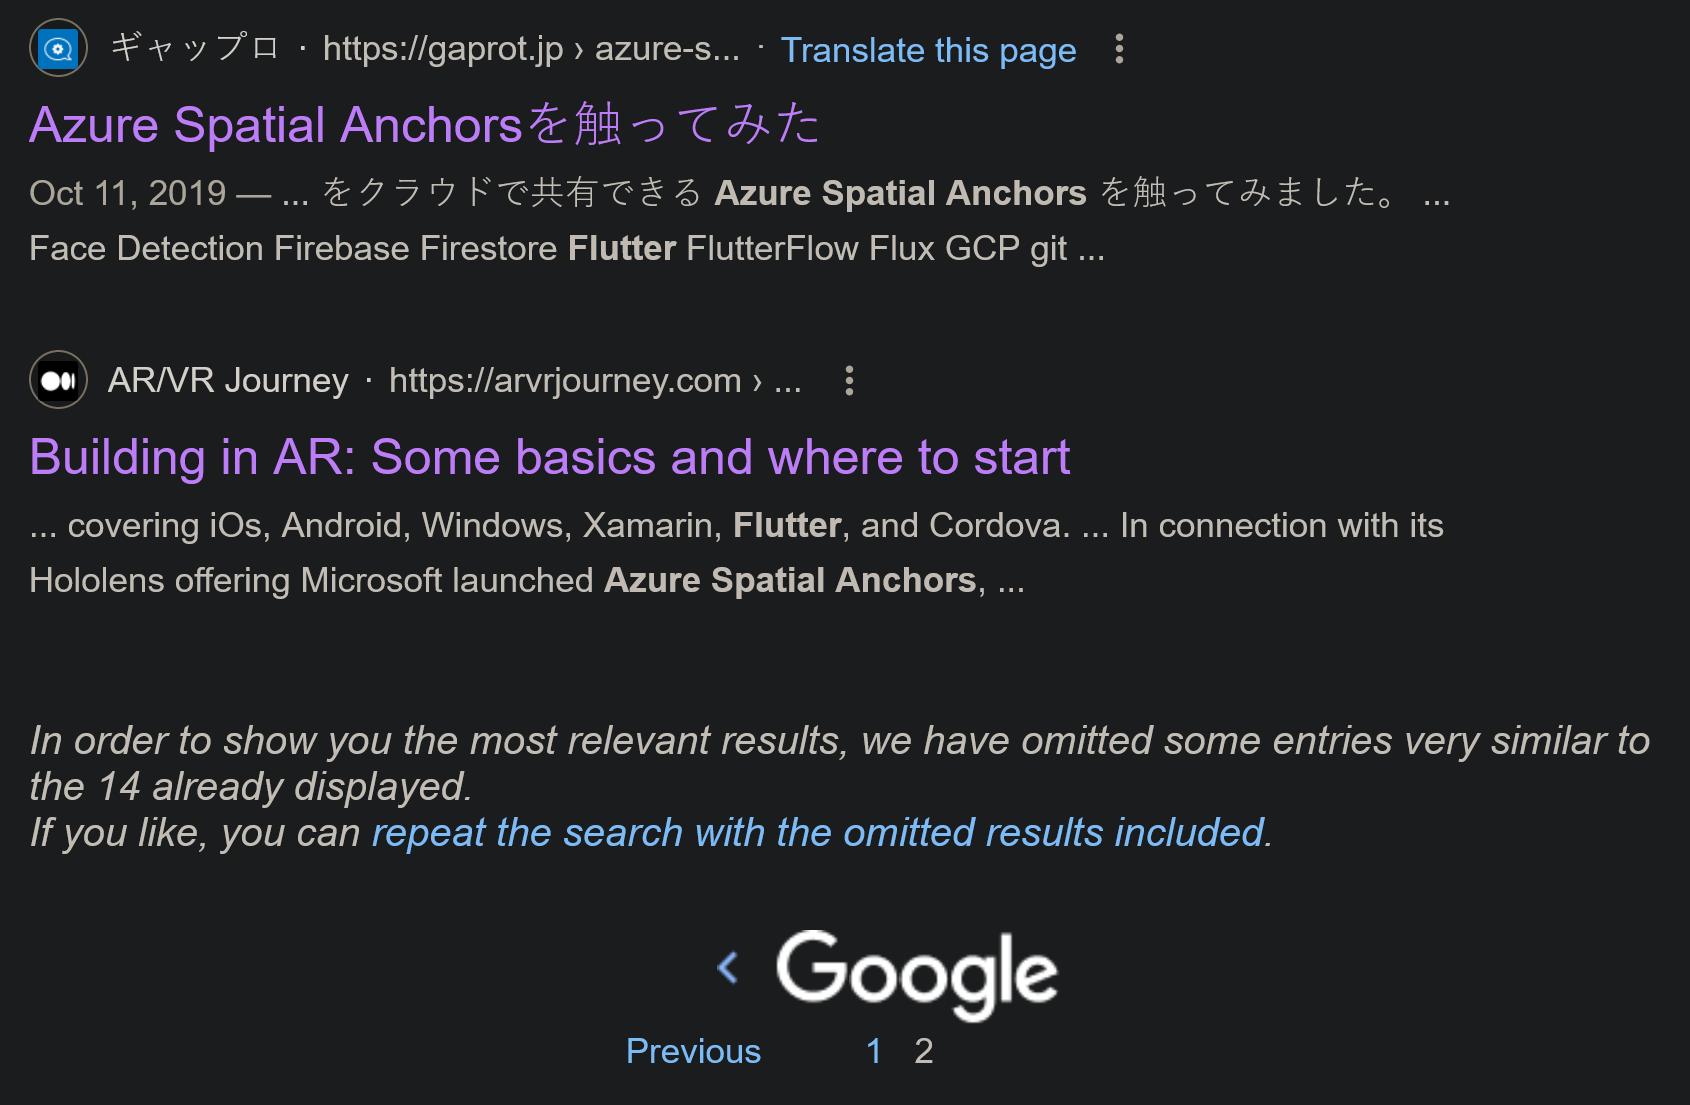
\includegraphics[width=.8\textwidth]{asa_flutter_search_today}
  \caption[Ricerca esatta Flutter e ASA 8 febbraio]{All'otto febbraio 2023 non si notano miglioramenti: solo 14 risultati rilevanti, alcuni in lingua giapponese, mostrano quando sia difficile trovare informazioni sull'argomento.}
  \label{fig:search2}
\end{figure}

Questa situazione ha significato dover risolvere tutti i problemi incontrati senza poter fare affidamento su alcun aiuto esterno e ha quindi esacerbato ulteriormente l'approccio \textit{trial-and-error} di cui si è parlato nella sezione \ref{sec:pianificazione}.

%************************************************************************************************************

\section{Soddisfacimento obiettivi}
\subsection{Valutazione personale}
\subsection{Valutazione proponente}

\section{Competenze}
\subsection{Competenze acquisite}
\subsection{Competenze mancanti}
\subsubsection{Lacune corso di studi}
